\section{Παράλληλη υλοποίηση του Αλγόριθμου}

Στον Crimmins Speckle removal αλγόριθμο το μόνο που πρέπει να παραμένει σειριακό είναι η σειρά με την οποία κάνουμε τα περάσματα για την διόρθωση των pixel για κάθε κατεύθυνση. Για τον λόγο αυτό επέλεξα να παραλληλοποιήσω την συνάρτηση που είναι υπεύθυνη για αυτά τα περάσματα. Έκανα την εξωτερική for loop παράλληλη έτσι ώστε να χωριστεί η εικόνα σε $\nicefrac{\Large n}{\Large p}$ κομμάτια όπου n οι γραμμές της εικόνας και p οι πυρήνες του συστήματος.

\begin{minted}[breaklines, breaksymbolright={}, breaksymbolleft={}, bgcolor=paraiso-light]{c}
void pass_func_par(uint8_t *image, uint8_t *tmp_image, uint32_t width,
    uint32_t height, int dx, int dy,
    uint8_t (*pass_logic_func)(uint8_t, uint8_t, uint8_t), int chunk)
{
    #pragma omp parallel for schedule(static, chunk)
    for(int y = 1; y < height - 1; y++) {
        uint8_t *row_a = tmp_image + (y-dy) * width;
        uint8_t *row_b = tmp_image + y * width;
        uint8_t *row_c = tmp_image + (y+dy) * width;
        uint8_t *row_out = image + y * width;

        for(int x = 1; x < width - 1; x++) {
            uint8_t a = row_a[x-dx];
            uint8_t b = row_b[x];
            uint8_t c = row_c[x+dx];

            b = pass_logic_func(a, b, c);

            row_out[x] = (b < 0) ? 0 :
                (b > 255) ? 255 :
                 b;
        }
    }
}
\end{minted}

Σημαντικό εδώ είναι οτί για τον pxeon2, πριν το τρέξουμε τον παράλληλο αλγόριθμο, πρέπει να θέσουμε τις μεταβλητές συστήματος \verb|OMP_PLACE=cores|, \verb|OMP_PROC_BIND=close|. Ο pxeon2 έχει τέσσερις φυσικούς Intel Xeon Gold 5218 επεξεργαστές ο κάθε ένας με την δικιά του μνήμη και δικιά του cache. Η μεταβλητές αυτές απλά λένε στο openmp να αρχίζει να γεμίζει πρώτα τα threads του ίδιου επεξεργαστή και να μην τα διανέμει ομοιόμορφα σε όλους. Αυτό μας διασφαλίζει ότι τα δεδομένα που χρειάζεται κάθε thread είναι κοντά τους οπότε δεν έχουμε μείωση του χρόνου γιατί πρέπει να επικοινωνήσουν διαφορετικοί επεξεργαστές μεταξύ τους όλη την ώρα. \cite{klemm2023advanced}, \cite{vanderpas2021numa}\\

Για να μπορώ να ελέγξω ότι τα αποτελέσματα του σειριακού και του παράλληλου αλγόριθμου είναι ίδια, έφτιαξα μια συνάρτηση (\verb|image_validator|) που περνάει τις δύο εικόνες και τις ελέγχει pixel προς pixel αν είναι ίδιες.

\newpage
\section{Πειραματικά αποτελέσματα OpenMP}

\begin{table}[htbp]
    \centering
    \begin{subtable}[t]{0.48\textwidth}
        \centering
        \pgfplotstabletypeset[
        col sep=tab,
        header=true,
        columns={threads,{lena256.raw/1 (serial)},{lena256.raw/1 (parallel)},{lena256.raw/1 (speedup)}},
        columns/threads/.style={column name=CPUs},
        columns/{lena256.raw/1 (serial)}/.style={column name=Ts,fixed,precision=4},
        columns/{lena256.raw/1 (parallel)}/.style={column name=Tp,fixed,precision=4},
        columns/{lena256.raw/1 (speedup)}/.style={column name=Sp,fixed,precision=2},
        column type=c,
        every first column/.style={column type=|c},
        column type/.add={|}{|},
        every head row/.style={
            before row=\hline,
            after row=\hline
        },
        every row/.style={
            before row=\hline
        },
        every last row/.style={
            after row=\hline
        }
        ]{./data/result_f1.csv}
        \caption{lena256.raw with 1 iteration}
    \end{subtable}%
    \hfill
    \begin{subtable}[t]{0.48\textwidth}
        \centering
        \pgfplotstabletypeset[
        col sep=tab,
        header=true,
        columns={threads,{mountain1024.raw/1 (serial)},{mountain1024.raw/1 (parallel)},{mountain1024.raw/1 (speedup)}},
        columns/threads/.style={column name=CPUs},
        columns/{mountain1024.raw/1 (serial)}/.style={column name=Ts,fixed,precision=4},
        columns/{mountain1024.raw/1 (parallel)}/.style={column name=Tp,fixed,precision=4},
        columns/{mountain1024.raw/1 (speedup)}/.style={column name=Sp,fixed,precision=2},
        column type=c,
        every first column/.style={column type=|c},
        column type/.add={|}{|},
        every head row/.style={
            before row=\hline,
            after row=\hline
        },
        every row/.style={
            before row=\hline
        },
        every last row/.style={
            after row=\hline
        }
        ]{./data/result_f1.csv}
        \caption{mountain1024.raw with 1 iteration}
    \end{subtable}

    \vspace{8pt}

    \begin{subtable}[t]{0.48\textwidth}
        \centering
        \pgfplotstabletypeset[
        col sep=tab,
        header=true,
        columns={threads,{mountain4096.raw/1 (serial)},{mountain4096.raw/1 (parallel)},{mountain4096.raw/1 (speedup)}},
        columns/threads/.style={column name=CPUs},
        columns/{mountain4096.raw/1 (serial)}/.style={column name=Ts,fixed,precision=4},
        columns/{mountain4096.raw/1 (parallel)}/.style={column name=Tp,fixed,precision=4},
        columns/{mountain4096.raw/1 (speedup)}/.style={column name=Sp,fixed,precision=2},
        column type=c,
        every first column/.style={column type=|c},
        column type/.add={|}{|},
        every head row/.style={
            before row=\hline,
            after row=\hline
        },
        every row/.style={
            before row=\hline
        },
        every last row/.style={
            after row=\hline
        }
        ]{./data/result_f1.csv}
        \caption{mountain4096.raw with 1 iteration}
    \end{subtable}%
    \hfill
    \begin{subtable}[t]{0.48\textwidth}
        \centering
        \pgfplotstabletypeset[
        col sep=tab,
        header=true,
        columns={threads,{mountain30000.raw/1 (serial)},{mountain30000.raw/1 (parallel)},{mountain30000.raw/1 (speedup)}},
        columns/threads/.style={column name=CPUs},
        columns/{mountain30000.raw/1 (serial)}/.style={column name=Ts,fixed,precision=4},
        columns/{mountain30000.raw/1 (parallel)}/.style={column name=Tp,fixed,precision=4},
        columns/{mountain30000.raw/1 (speedup)}/.style={column name=Sp,fixed,precision=2},
        column type=c,
        every first column/.style={column type=|c},
        column type/.add={|}{|},
        every head row/.style={
            before row=\hline,
            after row=\hline
        },
        every row/.style={
            before row=\hline
        },
        every last row/.style={
            after row=\hline
        }
        ]{./data/result_f1.csv}
        \caption{mountain30000.raw with 1 iteration}
    \end{subtable}
\end{table}

\begin{figure}[H]
    \centering
    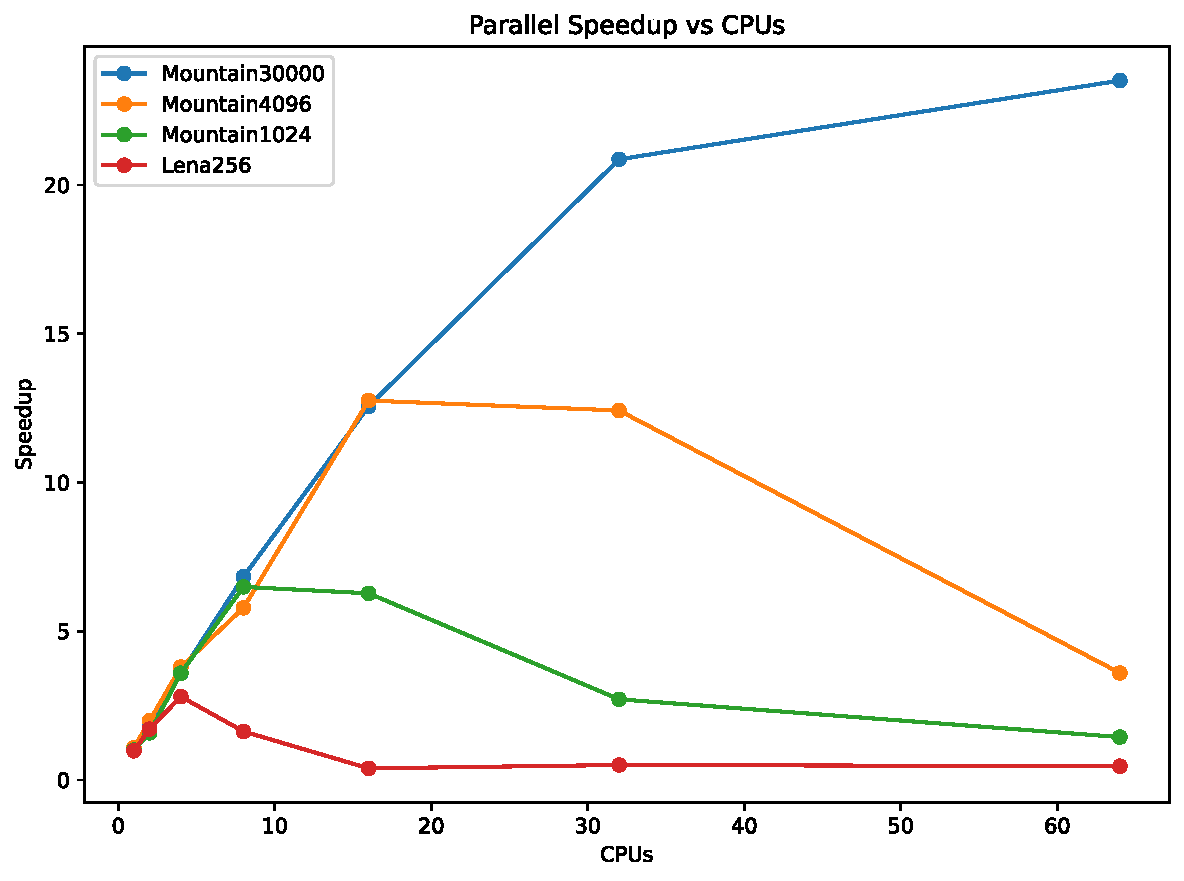
\includegraphics[width=0.8\linewidth]{./pics/speedupPlot.pdf}
    \caption{Speedup ανα Cores για διαφορετικά μεγέθους προβλήματα}
\end{figure}

Μπορούμε να παρατηρήσουμε ότι για μικρές εικόνες (μικρό μεγέθους πρόβλημα) το speedup αρχίζει να μειώνεται όσο αυξάνονται οι πυρήνες. Αυτό συμβαίνει γιατί οι γραμμές που παίρνει κάθε πυρήνας μειώνονται πολύ, σε βαθμό που ο έξτρα κώδικας που χρειάζεται ο παράλληλος αλγόριθμος για να κληθούν οι διαφορετικοί πυρήνες και να συγχρονιστούν προκαλούν την μείωση της απόδοσης του. Όσο μεγαλώνουν οι εικόνες (μεγαλώνει το μέγεθος του προβλήματος) ο κάθε πυρήνας έχει περισσότερες γραμμές να επεξεργαστεί οπότε η απόδοση αρχίζει να μειώνεται για μεγαλύτερο πλήθος πυρήνων. Για την εικόνα \verb|mountain30000|, που έχει πάρα πολλές γραμμές, δεν μπορούμε να δούμε με τους 64 πυρήνες μείωση του speedup.\\

Σημείωση, ότι τα πειραματικά αποτελέσματα πάρθηκαν ενώ έτρεχε στον pxeon2 ένα άλλο πρόγραμμα που χρησιμοποιούσε σχεδόν 90\% του επεξεργαστή, οπότε τα αποτελέσματα θα μπορούσαν να είναι και καλύτερα.
